\chapter{MetaSRA web interface } \label{app:website}

We developed a web interface website to enable querying the RNA-seq data in the SRA using the MetaSRA-mapped ontology terms, thereby facilitating discovery of public RNA-seq data. Matt Ziegler was the lead developer; however, I worked alongside Matt in designing the interface to the website and performing user-interviews to assess usability.   The website presents a number of features that take advantage of the MetaSRA schema discussed in Chapter~\ref{chap:2}:

\begin{itemize}
\item \textbf{Boolean queries:} We enable basic Boolean queries in which the user can specify a set of terms that the user requires for all search results as well as a set of terms that are used to filter search results (Fig~\ref{fig:webpage}).  Further, the user is able to filter their search results according to the MetaSRA's predicted sample-type category.
\begin{figure}[htbp]
\centering
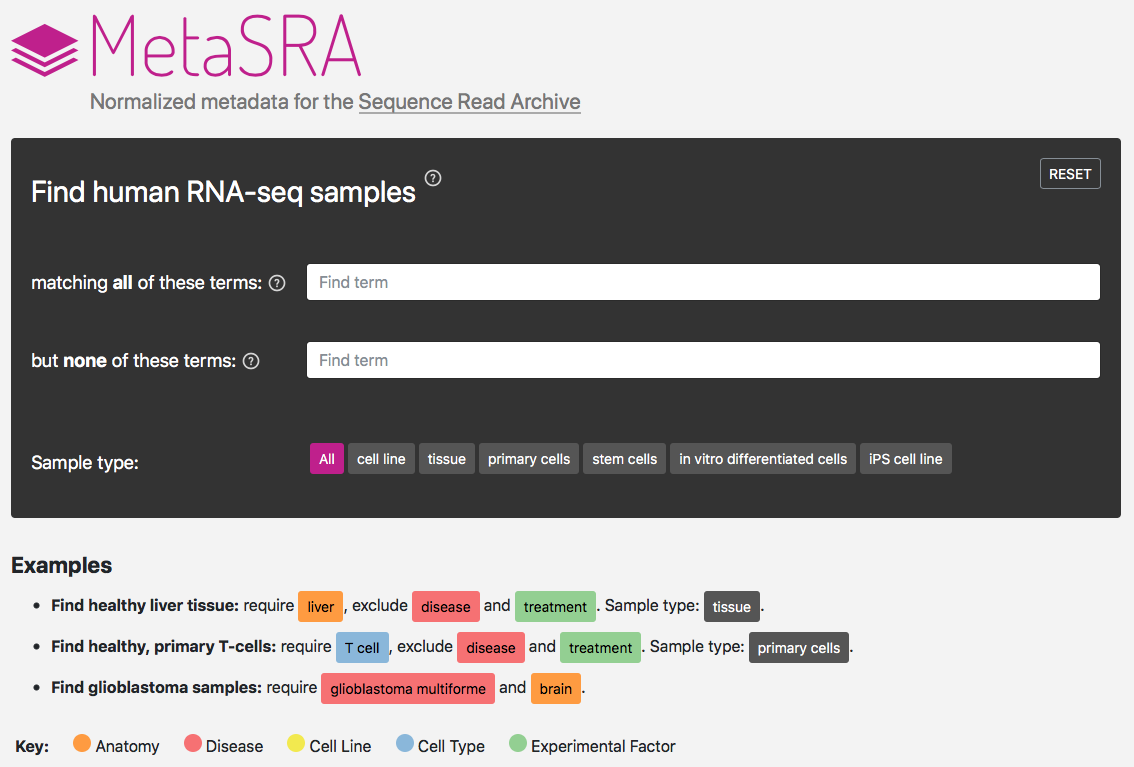
\includegraphics[width=12cm]{figures/web_page.png}  
\caption{\textbf{MetaSRA homepage.} A screenshot of the homepage for the MetaSRA website.}
\label{fig:webpage}
\end{figure}

\item \textbf{Ontology-based autocomplete}: The website requires that the user queries the metadata using ontology terms; however, this design-choice requires that users know what terms exist in the ontology \textit{a priori}.  This is often an unreasonable expectation of users. Therefore, we implemented an autocomplete feature (also called ``search suggestions") in order to help the user formulate their query using valid ontology terms. As the user is typing a query, a drop down menu appears with suggested ontology terms that may match the concept that the user has in mind.  Furthermore, each of these search-suggestions also presents ancestral terms (i.e. more general terms) and descendent terms (i.e. more specific terms) in order to further help the user discover queryable terms  (Fig.~\ref{fig:autocomplete}).  
\begin{figure}[htbp]
\centering
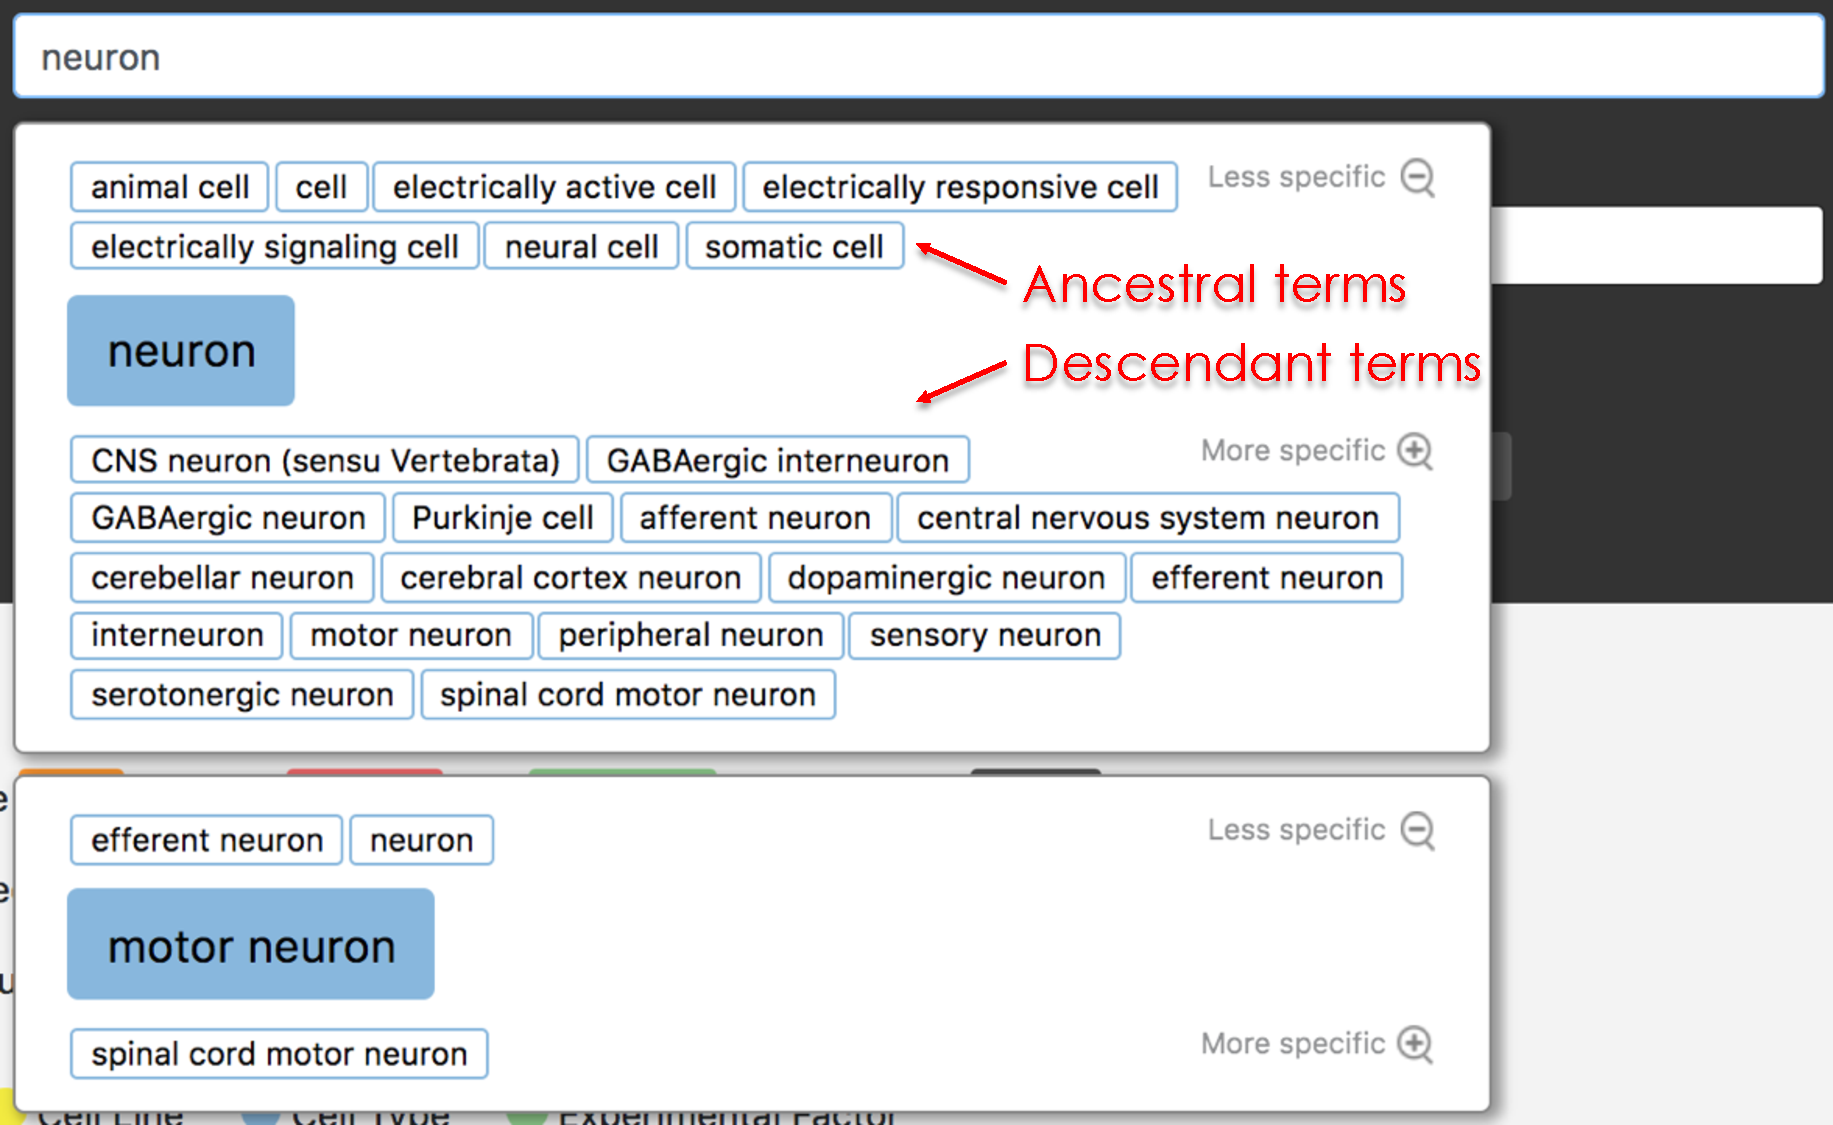
\includegraphics[width=12cm]{figures/autocomplete.pdf}  
\caption{\textbf{Autocomplete.} A screenshot of the autocomplete, search-suggestions that appear when the user types the query ``neuron".}
\label{fig:autocomplete}
\end{figure}

\item \textbf{Sample-set summaries:} We group the search-results by samples that all share identical metadata (and thus, also share identical mapped ontology terms) (Fig.~\ref{fig:search_results}).  This format avoids overwhelming the user with redundant search results. 
\begin{figure}[htbp]
\centering
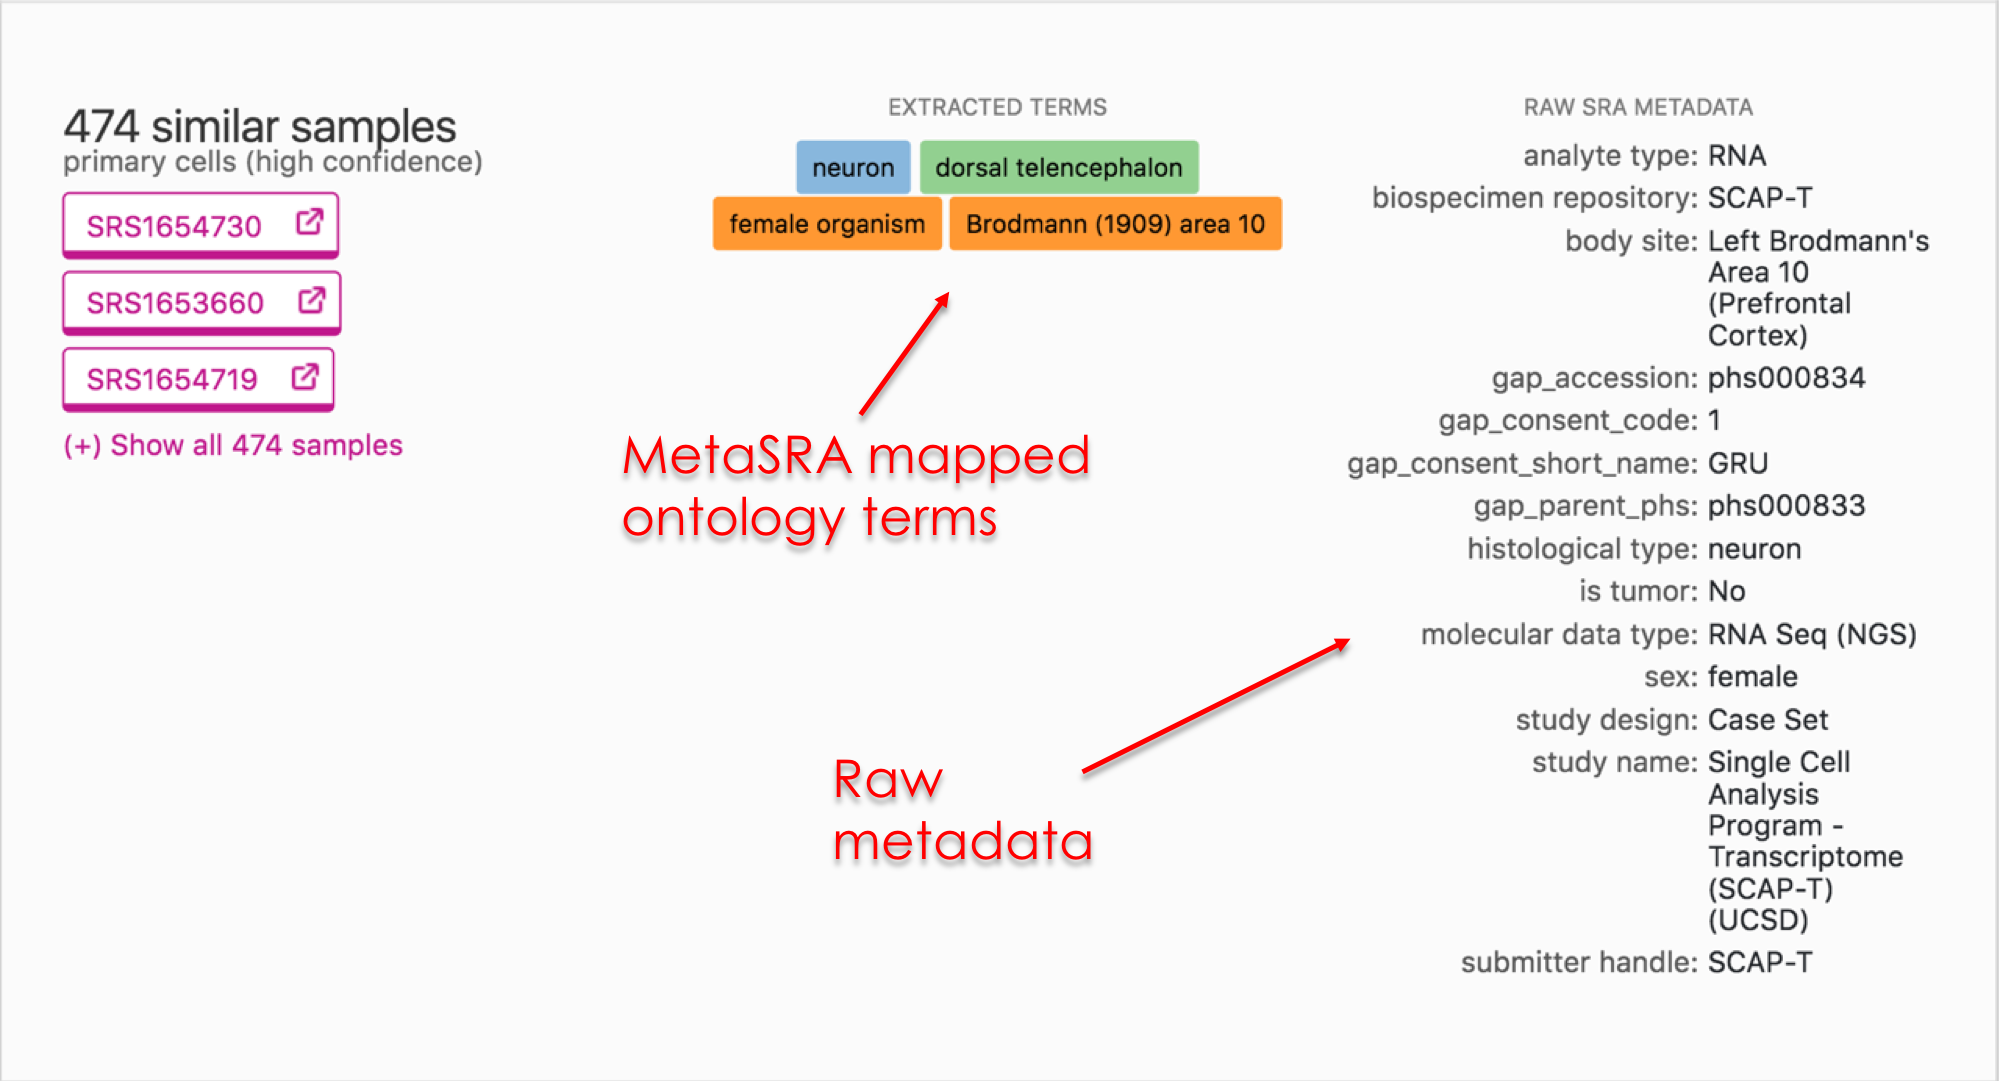
\includegraphics[width=12cm]{figures/search_results.png}
\caption{\textbf{Search results.} A screenshot of a set of samples returned by the query "neuron". These samples all share the same metadata and therefore are grouped into a single entry.  For each such group, we display the mapped ontology terms along with the original, raw metadata.}
\label{fig:search_results}
\end{figure}


\item \textbf{Search result term-clouds:} An important concern that users may have when querying the public data are co-occurring terms/phenotypes of the search results. For example, a user who is querying for samples from patients with diabetes, may wish to know about other characteristics of the search results such their cell type or tissue of origin.  To summarize this information, we present a ``term-cloud" of all terms that frequently co-occur with the search results (Fig.~\ref{fig:term_cloud}). Furthermore, the user can use the term cloud to further refine their search by selecting terms to further filter their results. 

\begin{figure}[htbp]
\centering
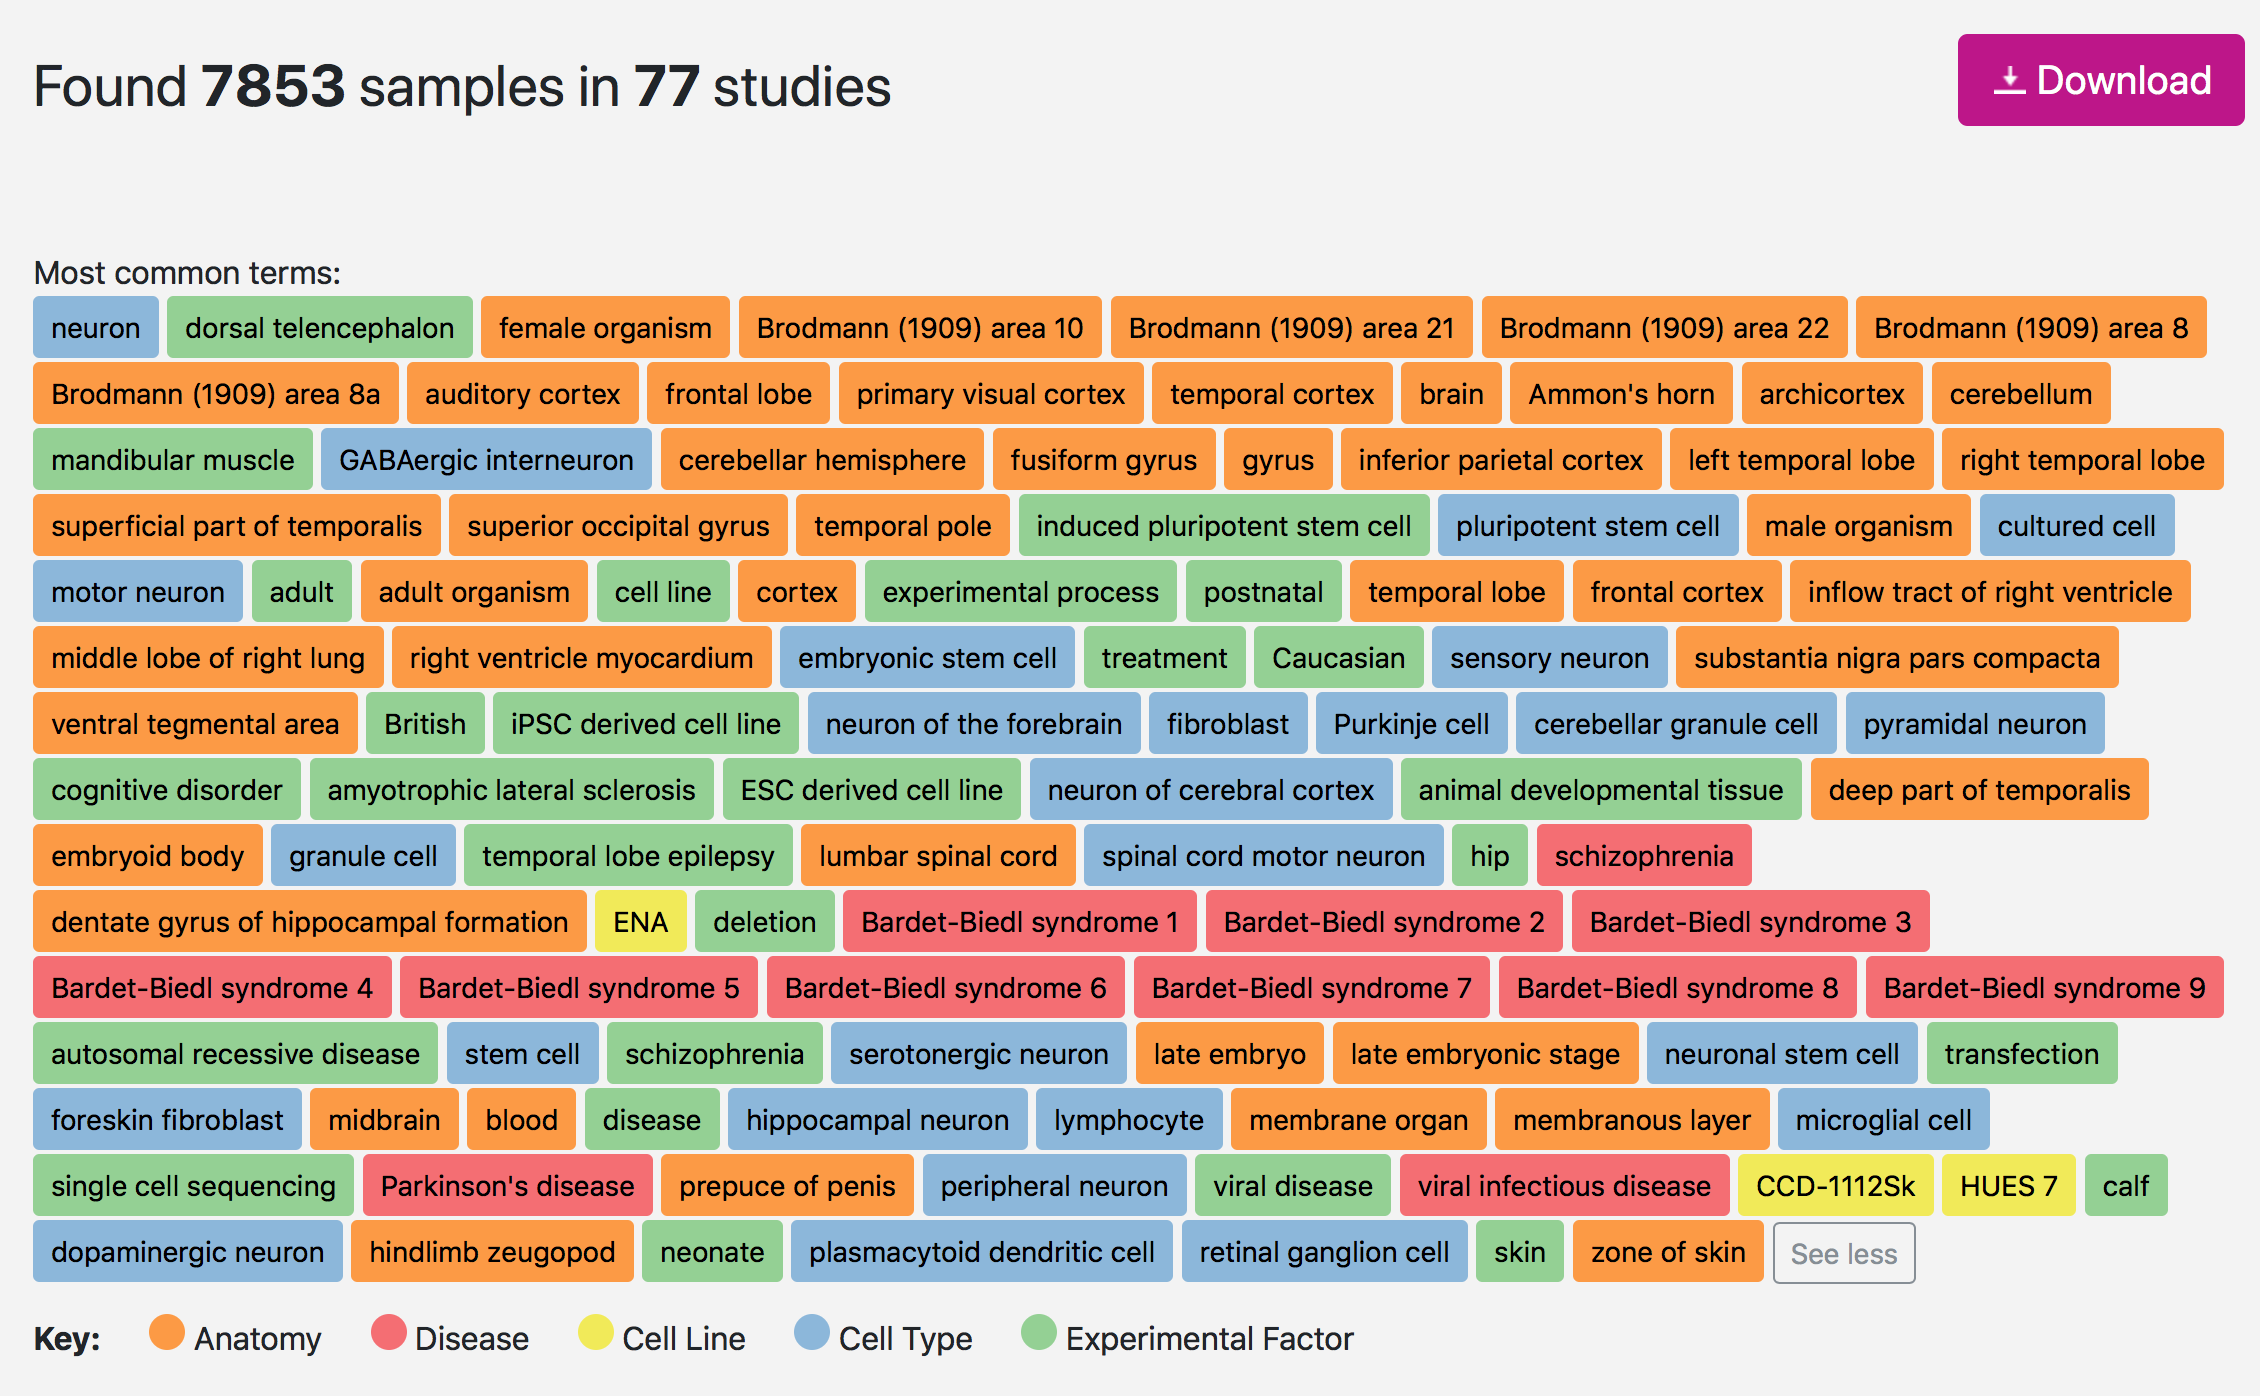
\includegraphics[width=12cm]{figures/term_cloud.png}
\caption{\textbf{Term cloud.} A screenshot of a the search results term cloud for the query "neuron".}
\label{fig:term_cloud}
\end{figure}

\end{itemize}





